\documentclass[12pt,a4paper]{article}
\usepackage[utf8]{inputenc}
\usepackage{amsmath}
\usepackage{amsfonts}
\usepackage{amssymb}
\usepackage{tabularx}
\usepackage{booktabs,dcolumn}
\usepackage{bbm}
\usepackage{natbib}
\setlength{\bibsep}{0.0pt}
\usepackage{graphicx}
\usepackage{setspace}
\usepackage{geometry}
\usepackage{array}
\usepackage[labelformat=simple]{subcaption}
\usepackage{setspace}
\usepackage[titletoc]{appendix}
\usepackage{changepage}
\usepackage{footmisc}
\usepackage{authblk}
\usepackage[disable, colorinlistoftodos,backgroundcolor=white, bordercolor=red, textcolor=red, textsize=tiny]{todonotes}
%\usepackage[whole]{bxcjkjatype} % 日本語
\usepackage{pdfpages}
\usepackage{subcaption}
\usepackage{comment}
%\usepackage{url} % 文献でのURL表示

\usepackage{lscape}
\usepackage{pdflscape}
\usepackage{rotating}

\usepackage{color}
\definecolor{MyBlue}{rgb}{0,0,0.6}
\usepackage[bookmarks=true,%
bookmarksnumbered=true,%
colorlinks=true,%
linkcolor=MyBlue,%
citecolor=MyBlue,%
filecolor=MyBlue,%
urlcolor=MyBlue%
]{hyperref}

\onehalfspacing
\bibpunct{(}{)}{;}{a}{}{;}
\geometry{top=2cm, bottom=2cm, left=3cm, right=3cm}
\newcolumntype{Z}{>{\centering\arraybackslash}X}
\abovecaptionskip=-2pt
\setlength{\marginparwidth}{2cm} % for todonotes

\title{\vspace{-0ex}朝ごはんと成績の相関関係について \\ --Peanutsのデータを用いて\thanks{aaa}}

\author{Charlie Schultz
\thanks{Department of Comics. Email: michihito.ando@rikkyo.ac.jp}  \ \  古川知志雄
\textsuperscript\thanks{Department of Economics. Email:furukawa-chishio-gj@ynu.ac.jp}}

\date{\today}




\begin{document}
\renewcommand\footnotelayout{\small}

\maketitle

\vspace{-10pt}\begin{abstract}
\begin{spacing}{1}
\noindent 
本稿では、2020年前半期を中心に、新型コロナウイルス危機に対する日本の財政的対応を検証した。この時期の国の財政措置は、2019年度の2つの緊急対応策と2020年度の2つの補正予算であり、総額は約58兆円であり、GDPの10\%以上に達した。2回に渡る緊急対応策では感染対策や経済支援・教育支援が中心であったのに対し、第1次補正予算では特別定額給付金という個人・世帯への支援が最大の支出項目であり、第2次補正予算では労働者・事業所・企業支援や医療・介護提供体制の強化などに重点がシフトした。また第1次補正予算を巡る政治過程の中で、特別定額給付金は選別的給付案から普遍的給付案へと変化し、総額25.7兆円の第1次補正予算の約半分を占めるほどの規模となった。一方、第1次補正予算では、雇用調整助成金や持続化給付金や``Go To''キャンペーンを中心に、労働者・事業者・企業への支援にも約9兆円程度が充当された。また本稿では、地方自治体の休業協力金の政策形成過程や既存の社会保障制度における新型コロナ対応についても整理した。\\

\noindent\textbf{JEL classification}: E62, H12, H53, H60, H84  \\
\noindent\textbf{Keywords}: 新型コロナウイルス、緊急経済対策、2020年度補正予算、第1次補正予算、特別定額給付金
\end{spacing}
\end{abstract}

\newpage

\section{相関関係の分析} 


\begin{figure}
\centering
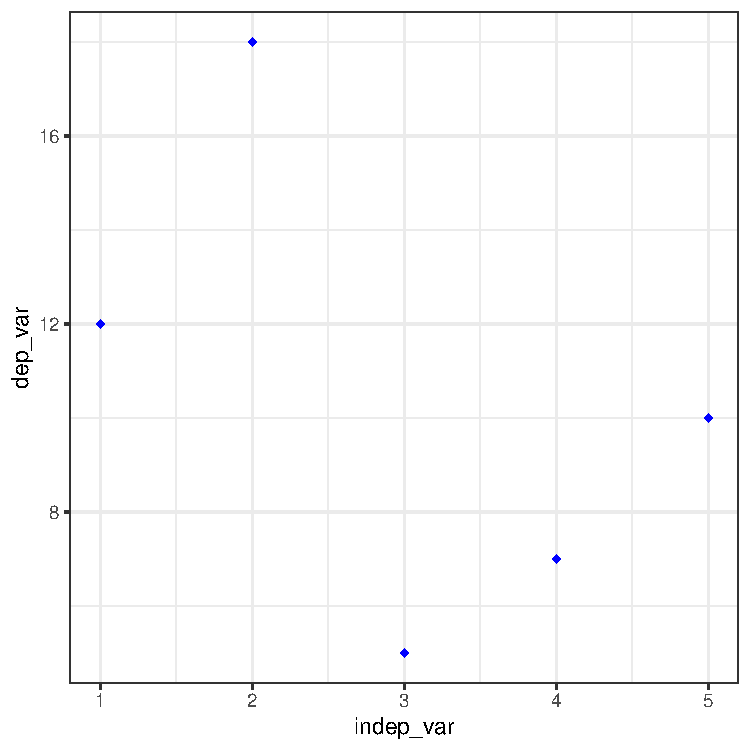
\includegraphics[width=7cm]{04_analyze/scatter_regress/figure/figure.pdf}

\label{fig:img1}
\caption{Bare figure}
\end{figure}


あいうえお
このフォントはみやすいだろうか。

% \begin{figure}
% \centering
% \includegraphics[width=7cm]{Unemployment_Insurance.pdf}

% \label{fig:img2}
% \caption{Simulation}
% \end{figure}

% \begin{table}
% \let\center\empty
% \let\endcenter\relax
% \centering
% \resizebox{.8\width}{!}{\input{subfolder/table}}
% \end{table}

\bibliographystyle{econ} 
\bibliography{covid19_fiscal}

\end{document}